\section{The recognition model}
\label{sec:model}

\begin{figure}[t]
\centering
% Architecture / dataflow diagram.
% Requires: tikz with arrows.meta, positioning (loaded in main.tex).
\begin{tikzpicture}[
  font=\small,
  box/.style={draw=prule, fill=white, rounded corners=2pt, line width=0.7pt,
              minimum height=11mm, text width=30mm, inner sep=4pt,
              align=center},
  learned/.style={box, draw=pblue, fill=pblue!7},
  search/.style={box, draw=pviolet, fill=pviolet!7},
  data/.style={box, draw=pgrey!45, fill=pbox},
  gate/.style={box, draw=porange, fill=porange!8},
  ar/.style={-{Stealth[length=4pt]}, draw=pgrey, line width=0.7pt},
  lbl/.style={font=\scriptsize, color=pgrey, inner sep=2pt},
]

% row 1 --- capture and preprocessing
\node[data]                          (cam)   at (0,0)      {webcam\\[-2pt]\scriptsize 30\,fps JPEG};
\node[data, right=7mm of cam]        (yolo)                {YOLOv8n crop\\[-2pt]\scriptsize every 10th frame,\\[-3pt]\scriptsize median $+$ interpolate};
\node[data, right=7mm of yolo]       (stack)               {$96{\times}96$, 4 channels\\[-2pt]\scriptsize RGB $+$ $\Delta$luma};

% row 2 --- the network
\node[learned, below=9mm of cam]     (enc)                 {frame encoder\\[-2pt]\scriptsize 4 conv, shared\\[-3pt]\scriptsize $\to\mathbb{R}^{128}$ per frame};
\node[learned, right=7mm of enc]     (tcn)                 {dilated TCN\\[-2pt]\scriptsize 4 blocks $d\!=\!1,2,4,8$\\[-3pt]\scriptsize RF 61 fr ($2.0$\,s)};
\node[learned, right=7mm of tcn]     (head)                {$1{\times}1$ head\\[-2pt]\scriptsize 13 logits / frame\\[-3pt]\scriptsize 12 turns $+$ blank};

% row 3 --- the two searches and the gate
\node[search, below=9mm of enc]      (beam)                {CTC prefix beam\\[-2pt]\scriptsize search over \emph{frames}\\[-3pt]\scriptsize $\Rightarrow$ move string};
\node[search, right=7mm of beam]     (recon)               {group decode\\[-2pt]\scriptsize beam over edits\\[-3pt]\scriptsize must reach solved};
\node[gate,   right=7mm of recon]    (gate)                {count gate\\[-2pt]\scriptsize QTM floor $=32$\\[-3pt]\scriptsize verified / review / reject};

% row 4 --- side inputs
\node[data, below=9mm of beam, draw=paqua, fill=paqua!8] (ble)
      {\textbf{BLE cube}\\[-2pt]\scriptsize labels + ground truth,\\[-3pt]\scriptsize \emph{never an input}};
\node[data, below=9mm of recon]      (states)              {known endpoints\\[-2pt]\scriptsize server scramble\\[-3pt]\scriptsize $+$ solved};

% arrows
\draw[ar] (cam)   -- (yolo);
\draw[ar] (yolo)  -- (stack);
\draw[ar] (stack.south) -- ++(0,-4.5mm) -| (enc.north);
\draw[ar] (enc)   -- (tcn);
\draw[ar] (tcn)   -- (head);
\draw[ar] (head.south)  -- ++(0,-4.5mm) -| (beam.north);
\draw[ar] (beam)  -- node[lbl, above]{transcript}   (recon);
\draw[ar] (recon) -- node[lbl, above]{repaired}     (gate);
\draw[ar] (states.north) -- (recon.south);
\draw[ar, draw=paqua, dashed] (ble.east) -- (states.west);
\draw[ar] (beam.east) .. controls +(10mm,-9mm) and +(-14mm,-9mm)
          .. node[lbl, below, pos=0.55]{move \emph{count}} (gate.south);

\end{tikzpicture}

\caption{The pipeline. Everything left of the dashed line is per-frame and
learned; everything right of it is a search. The smart cube (bottom) supplies
labels during data collection and ground truth during evaluation, and is
absent at inference.}
\label{fig:pipeline}
\end{figure}

\subsection{Architecture}
\label{sec:arch}

The network is deliberately small: \NParams\ parameters, trained in minutes,
chosen so that ``wrong architecture'' and ``not enough data'' stay
distinguishable. With ${\sim}5{,}000$ labelled turns from one person, a large
recurrent model over raw frames has ample capacity to memorise grip and
lighting.

\paragraph{Frame encoder.} Four strided $3\times3$/$5\times5$ convolutions
with batch-norm and ReLU take $4\times96\times96 \rightarrow 128\times6\times6$,
followed by global average pooling: one 128-dimensional vector per frame,
weights shared across frames. Pooling away the spatial dimensions is a real
commitment --- it discards \emph{where} on the cube the motion was --- and it
is defensible only because the temporal difference channel already encodes
the pattern of a turn rather than its location. It is also the most obvious
thing to revisit (\cref{sec:gap}).

\paragraph{Temporal convolutional network.} Four residual blocks, each two
$3$-wide dilated 1-D convolutions at dilations $1,2,4,8$ with `same' (centred)
padding. The receptive field is
\begin{equation}
1 + \sum_{d\in\{1,2,4,8\}} 4d \;=\; 61 \text{ frames} \;\approx\; 2.03\,\text{s
at 30\,fps,}
\end{equation}
i.e.\ each output frame sees roughly one second either side. The network is
therefore \textbf{non-causal by design}, which suits the intended product
flow (buffer the solve, analyse it afterwards) and would need causal padding
and an accuracy sacrifice at the leading edge for true streaming.

\paragraph{Heads.} A $1\times1$ convolution maps the 128-channel trunk to 13
logits per frame: 12 quarter turns plus blank. A second $1\times1$ head
producing a single onset logit is retained from the earlier architecture and
is trained with weight $0$ in the shipped configuration; it is what the
peak-picking arm in \cref{sec:ablation} uses.

Being fully convolutional in time means the model trains on fixed-length
clips and runs a whole session in one pass. In practice a session is chunked
at 480 frames with 30 frames of context on each side that are then
discarded, because a chunk boundary with zero padding produces a band of
${\sim}60$ unreliable scores --- over 10\% of a session's output, exactly
where symbols are being read off.

\subsection{Two supervision regimes}
\label{sec:supervision}

The same trunk was trained two ways, and the difference is the most
consequential design decision in the project.

\paragraph{(a) Alignment supervision.} Each BLE onset becomes a Gaussian
bump ($\sigma = 1$ frame) in a per-frame target; the onset head is trained
with BCE, the class head with cross-entropy at labelled frames. At inference,
peaks are picked out of the onset score (threshold, minimum separation), each
peak becomes a move, and the class head is read at the peak frame.

\paragraph{(b) CTC.} The 13th column becomes a blank, the loss is
$-\log p(\ell^\star \mid x)$ from \cref{eq:ctcmarginal}, and nothing ever
tells the network \emph{where} a move was.

Regime (a) uses information that regime (b) throws away, which sounds like a
straightforward advantage. The argument for (b) is that the discarded
information is \emph{partly wrong exactly where the pipeline fails}:
\CorpusCrowdedTwo\% of turns land within two frames of a neighbour and
\CorpusSameFrame\% cannot be assigned distinct frames at all
(\cref{sec:capture}), and those crowded pairs are the same population that
peak-picking loses to merged humps. CTC is indifferent to both.

\paragraph{The deeper problem with (a) is architectural, not statistical.}
Peak-picking commits to a discrete candidate list \emph{before} any
downstream search runs. Every phantom and every miss in the pipeline is
created at that one line. A regrip hump that clears the threshold becomes a
phantom the group decoder must pay to delete; two onsets closer than the
minimum separation can never both be reported at all. CTC does not improve
that step, it removes it: the search runs over \emph{frames}, so ``is there a
move here'' is decided inside the search, weighed against everything else,
rather than greedily beforehand by a constant.
\Cref{sec:ablation} measures the swap.

\subsection{What the model actually emits}
\label{sec:posteriorgram}

\begin{figure}[t]
\centering
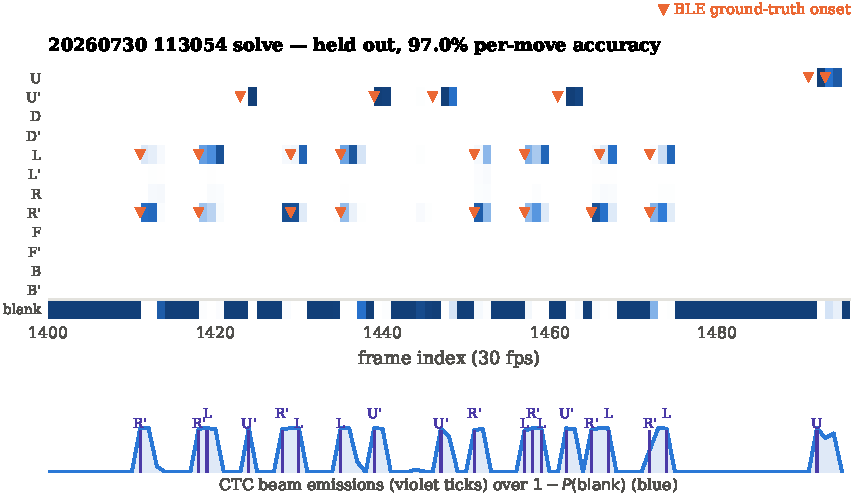
\includegraphics[width=\linewidth]{figures/fig_posteriorgram.pdf}\\[6pt]
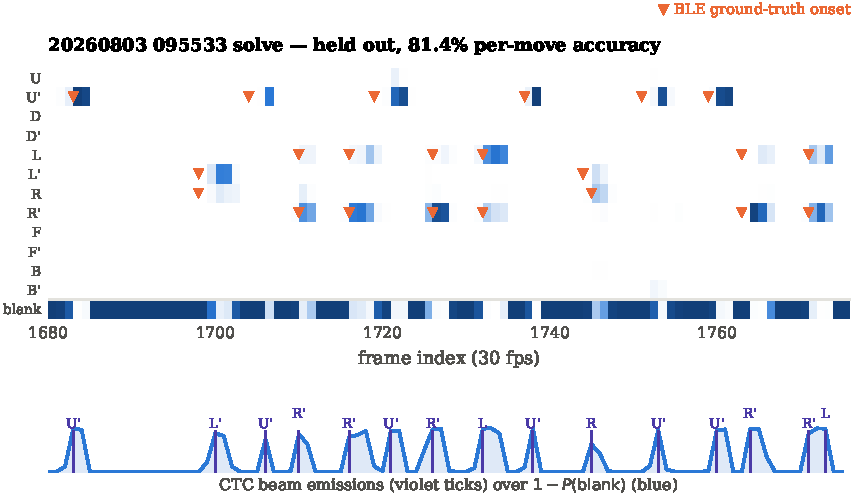
\includegraphics[width=\linewidth]{figures/fig_ctc_failure.pdf}
\caption{The 13-way per-frame posterior over 3.2\,s of two held-out
sessions, with BLE ground-truth onsets marked. \textbf{Top:} a session the
model reads well. The posterior is extremely peaky --- the network spends
${\sim}90$\% of frames confidently in blank and commits for one or two frames
per turn --- and every truth marker has a matching dark cell in its own row.
\textbf{Bottom:} a session it reads badly. The posterior is visibly softer
and several truth markers sit over rows with no committed mass at all;
those are the misses that dominate the error budget. Note in both panels
that emissions do not have to align with the markers, only to appear in the
right order: CTC is never told where a move was.}
\label{fig:posteriorgram}
\end{figure}

\Cref{fig:posteriorgram} is the most useful single picture of this system.
Two properties are worth reading off it.

First, \textbf{CTC produces a peaky posterior}, not a smooth one. This is a
well-known property of the objective --- the marginalisation in
\cref{eq:ctcmarginal} is happy to place all of a symbol's probability on one
frame --- and it has a practical consequence: the ``score'' of a move is not
a smooth confidence that can be thresholded, which is why the decoders in
\cref{sec:decode} search over frames rather than over thresholded peaks.

Second, \textbf{the failure mode is silence, not confusion}. In the lower
panel the model does not name turns wrongly so much as decline to name them.
That is consistent with the error decomposition in \cref{sec:main-results}
and it is why the group decoder --- whose cheap repair is substitution ---
has so little to work with.

\subsection{Augmentation}
\label{sec:aug}

Two families, both applied per clip.

\paragraph{Photometric.} Gain $\in[0.55,1.60]$, offset $\pm 30$, gamma
$\in[0.60,1.65]$, per-channel white balance $\in[0.86,1.16]$, saturation
$\in[0.65,1.35]$, per-frame gain wobble ($\sigma=0.03$), Gaussian noise
($\sigma$ up to 5), and with probability $0.15$ a 3-frame temporal box blur
simulating the longer exposure of a dim room. These ranges are roughly
3--4$\times$ wider than the original ones, widened after an evening take
scored 56\% against ${\sim}91\%$ on two morning takes.

\paragraph{Speed.} With probability $0.5$ a clip is time-warped by a factor
in $[1.2, 3.0]$, resampling $96\cdot s$ source frames down to 96. On a
2.4\,turns/s corpus a factor of 3 reaches ${\sim}7$\,turns/s.

Speed augmentation was introduced for an anticheat reason --- the count gate
needs the model not to under-count fast solves --- and the repository records
it as having ``zero validation cost''. \Cref{sec:ablation} shows that on a
never-seen holdout it is the largest single accuracy intervention on record.
This is the sharpest instance in the project of a recurring lesson:
\emph{validation MER did not rank these interventions, and the corpus's own
validation split was structurally incapable of doing so} because it is
same-day adjacent (\cref{sec:ladder}).

One practical note that cost a debugging session: with speed augmentation the
CTC loss escapes its all-blank plateau roughly four epochs later than
without. That is expected --- time-warped clips make the alignment problem
harder early --- and is not a bug, but it looks exactly like one.

\subsection{Training}

AdamW, learning rate $3\times10^{-4}$, weight decay $10^{-2}$, batch 8 clips
of 96 frames (3.2\,s) sampled at stride 24, gradient clipping at 5, mixed
precision, 60 epochs with patience 15. Model selection is by move error rate
on the held-out validation sessions, never by loss: per-frame loss is
dominated by the easy blank frames between moves, and a model can improve
its loss while getting worse at emitting exactly one symbol per turn.

\textbf{Session-level holdout is mandatory}, not optional. Clips from one
session overlap and share lighting, grip and background; a random clip split
reports memorisation. Every checkpoint in this report was trained with named
validation sessions.

Two seeds are trained for every configuration and both are always reported.
The two-seed spread on this metric is 0.5--3 points depending on regime, and
several interventions in the project's history were smaller than it.
